\documentclass[a4paper,11pt]{article}

\usepackage[utf8]{inputenc}
\usepackage[top=2cm, left = 2cm , right=2cm , bottom=2cm]{geometry}
\usepackage{amsmath}
\usepackage{graphicx}
\usepackage{float}
\usepackage{listings}
\usepackage[brazil]{babel}
\usepackage{multicol}

\usepackage{color}

\definecolor{mygreen}{rgb}{0,0.6,0}
\definecolor{mygray}{rgb}{0.5,0.5,0.5}
\definecolor{mymauve}{rgb}{0.58,0,0.82}

\lstset{
  backgroundcolor=\color{white},   % choose the background color; you must add
                                   % \usepackage{color} or \usepackage{xcolor};
                                   % should come as last argument
  basicstyle=\footnotesize,        % the size of the fonts
  breakatwhitespace=false,         % sets if automatic breaks should only happen
                                   % at whitespace
  breaklines=true,                 % sets automatic line breaking
  captionpos=b,                    % sets the caption-position to bottom
  commentstyle=\color{mygreen},    % comment style
  escapeinside={\%*}{*)},          % if you want to add LaTeX within your code
  extendedchars=true,              % lets you use non-ASCII characters; for
                                   % 8-bits encodings only, does not work with
                                   % UTF-8
  frame=single,	                 % adds a frame around the code
  keepspaces=true,                 % keeps spaces in text, useful for keeping
                                   % indentation of code (possibly needs
                                   % columns=flexible)
  keywordstyle=\color{blue},       % keyword style
  language=Matlab,                 % the language of the code
  numbers=left,                    % where to put the line-numbers; possible
                                   % values are (none, left, right)
  numbersep=5pt,                   % how far the line-numbers are from the code
  numberstyle=\tiny\color{mygray}, % the style that is used for the line-numbers
  rulecolor=\color{black},         % if not set, the frame-color may be changed
                                   % on line-breaks within not-black text
                                   % (e.g. comments (green here))
  showspaces=false,                % show spaces everywhere adding particular
                                   % underscores; it overrides
                                   % 'showstringspaces'
  showstringspaces=false,          % underline spaces within strings only
  showtabs=false,                  % show tabs within strings adding particular
                                   % underscores
  stepnumber=2,                    % the step between two line-numbers. If it's
                                   % 1, each line will be numbered
  stringstyle=\color{mymauve},     % string literal style
  tabsize=2,                       % sets default tabsize to 2 spaces
  title=\lstname                   % show the filename of files included with
                                   % \lstinputlisting; also try caption instead
                                   % of title
}

\pagestyle{plain}

\graphicspath{{./Imagens/}}

\begin{document}

\begin{center}
\textbf{Pré-relatório Experiência 3} \\
\hspace{5pt}
Prof. Marconi Kolm Madrid \\
EA722 - 2017/2
\end{center}

\begin{center}
Danilo Pereira Titato - RA 122541 \\
Giovani Granzotto Oliani - RA 146253 \\
Pedro Gabriel Calixto Mendonça - RA 118363 \\
\end{center}

\textbf{1.}

Função de transferência do controlador PD:
\begin{gather*}
    X_1 = G_p \cdot \left(k_p + k_ds\right) \cdot \left(R - X_1\right) \\
    X_1 \left[1 + G_p \cdot \left(k_p + k_ds\right)\right] =
        R \cdot G_p \cdot \left(k_p + k_ds\right) \\
    G_{PD} = \frac{X_1}{R} = \frac{\left(k_p + k_ds\right) \cdot G_p}
        {1 + \left(k_p + k_ds\right) \cdot G_p}
\end{gather*}

Função de transferência do controlador P\&D:
\begin{gather*}
    X_1 = G_p \cdot \left[k_p \cdot \left(R - X_1\right) -
        k_ds \cdot X_1\right] \\
    X_1 \left(1 + k_p G_p + k_ds \cdot G_p\right) = R \cdot k_p G_p \\
    G_{P\&D} = \frac{X_1}{R} = \frac{k_p G_p}
        {1 + \left(k_p + k_ds\right) \cdot G_p}
\end{gather*}

\textbf{2.} O \textit{script} usado em Matlab para obtenção dos póloes e zeros
dos controladores foi:

\begin{lstlisting}
% parametros iniciais
s = tf('s');

mc1 = 0.778;
mw1 = 4*0.500;
m1 = mc1 + mw1;

c1 = 2.94;
kv = 0.005;
khw = 14732;

k1 = 338.6;
deltak1 = 361.4;

kp = 0.08;
kd = 0.01;

% funcao de transferencia da planta
Gp = khw / (m1*s^2 + (c1+khw*kv)*s + k1);

% controlador PD
Hpd = (kp+kd*s)*Gp / (1 + (kp+kd*s)*Gp);

% controlador P&D
Hped = kp*Gp / (1 + (kp+kd*s)*Gp);

% calculo dos polos e zeros
pzmap(Hpd)
pzmap(Hped)
\end{lstlisting}

\pagebreak

Os gráficos obtidos foram:

\begin{figure}[H]
\centering
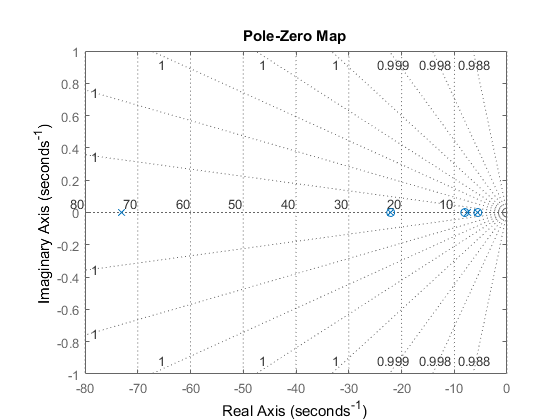
\includegraphics{pzmap-pd}
\caption{Lugar das raízes do controlador PD}
\end{figure}

\begin{figure}[H]
\centering
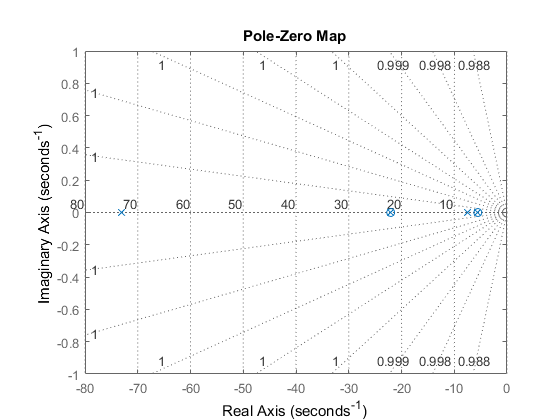
\includegraphics{pzmap-ped}
\caption{Lugar das raízes do controlador P\&D}
\end{figure}

\underline{Controlador PD}

\begin{multicols}{2}
    Pólos:
    \begin{itemize}
        \item -73.1375 $rad/s$
        \item -22.0448 $rad/s$
        \item -7.4672 $rad/s$
        \item -5.5290 $rad/s$
    \end{itemize}
\columnbreak
    Zeros:
    \begin{itemize}
        \item -22.0448 $rad/s$
        \item -8.0000 $rad/s$
        \item -5.5290 $rad/s$
    \end{itemize}
\end{multicols}

\underline{Controlador P\&D}

\begin{multicols}{2}
    Pólos:
    \begin{itemize}
        \item -73.1375 $rad/s$
        \item -22.0448 $rad/s$
        \item -7.4672 $rad/s$
        \item -5.5290 $rad/s$
    \end{itemize}
\columnbreak
    Zeros:
    \begin{itemize}
        \item -22.0448 $rad/s$
        \item -5.5290 $rad/s$
    \end{itemize}
\end{multicols}

\textbf{3.} \textbf{(a)}
O diagrama de blocos usado para implementar as condições iniciais do controlador
PD foi:

\begin{figure}[H]
\centering
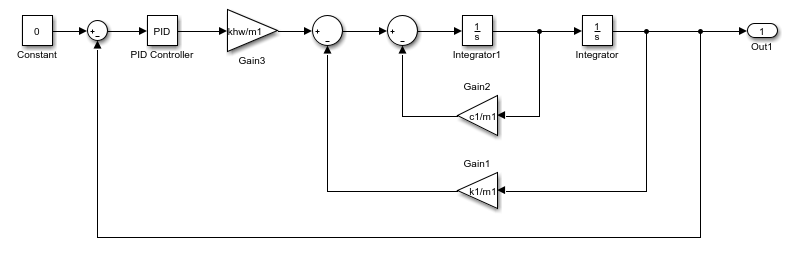
\includegraphics[scale=0.75]{diagrama-pd}
\end{figure}

Sua resposta temporal para entrada nula e condições iniciais
$x_1\left(0\right) = 1000$ counts, $\dot{x}_1\left(0\right) = 0$, foi:

\begin{figure}[H]
\centering
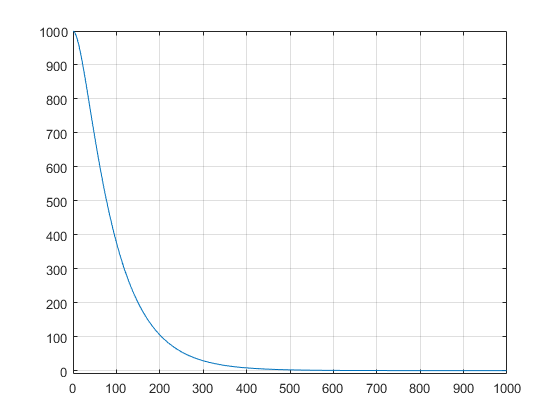
\includegraphics{exp03e03a-resposta-pd}
\end{figure}

\textbf{(b)}
O diagrama de blocos usado para implementar as condições iniciais do controlador
P\&D foi:

\begin{figure}[H]
\centering
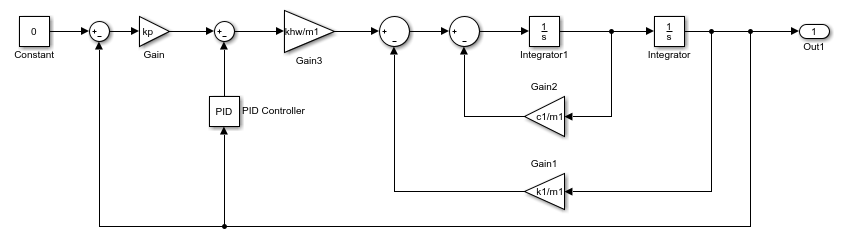
\includegraphics[scale=0.75]{diagrama-ped}
\end{figure}

Sua resposta temporal para entrada nula e condições iniciais
$x_1\left(0\right) = 1000$ counts, $\dot{x}_1\left(0\right) = 0$, foi:

\begin{figure}[H]
\centering
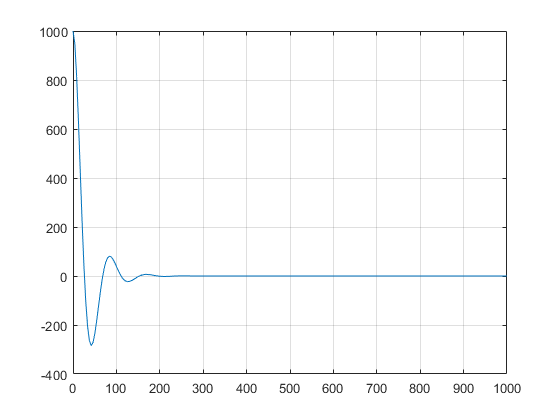
\includegraphics{exp03e03b-resposta-ped}
\end{figure}

Como visto, a resposta do controlador P\&D teve um tempo de subida
significativamente menor. A resposta do P\&D oscilou com um \textit{overshoot}
acentuado e seu regime se deu por volta de entre $200$ e $300ms$, enquanto o
regime do controlador PD se deu por volta de entre $500$ e $600ms$, com uma
resposta consideravelmente mais amortecida.

\pagebreak

\textbf{(c)}

\begin{figure}[H]
\centering
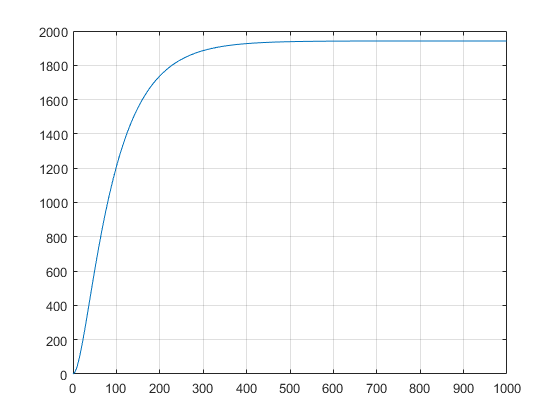
\includegraphics{exp03e03c-resposta-pd}
\caption{Resposta do controlador PD à entrada degrau}
\end{figure}

\begin{figure}[H]
\centering
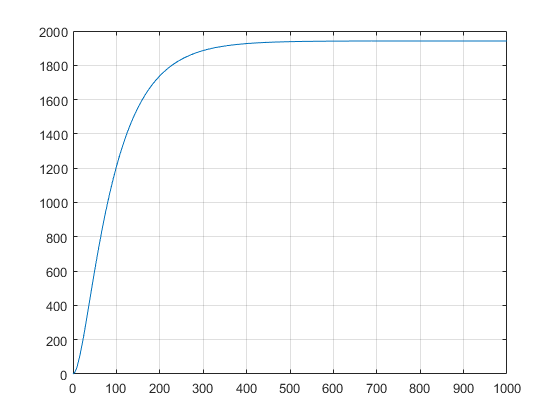
\includegraphics{exp03e03c-resposta-ped}
\caption{Resposta do controlador P\&D à entrada degrau}
\end{figure}

\end{document}